\chapter{Particle Physics}
\section{Coassification of Elementary Particles}
\subsection{Leptons}
These are simplest and elementary particle with no internal structure known. They are  affected by electromagnetic, weak and gravitational forces but not by strong interaction.\\
These are three pairs:\\
Electrons $(e), \operatorname{Muon}(\mu), \operatorname{Tauon}(\tau)$, Electron-neutrino $\left(v_e\right)$, Muon-neutrino $\left(v_\mu\right)$,
Tau-neutrino $\left(v_r\right)$.\\
They also have corresponding antiparticles.
\subsection{Baryons}
Protons and particles heavier than proton form this group. Proton $(p)$ and neutron $(n)$ are called nucleons and rests are called Hyperons.\\
$\text { Hyperons }$ are a special class of baryons characterized by a time decay of the order of $\approx 10^{-10} \mathrm{sec}$ and mass value intermediate between those of the neutrons and deuteron. Their decay time is very much greater than the time of their formation time $\left(\approx 10^{-23} \mathrm{sec}\right)$.\\\\
It is because of this unsolved problem that these particles along with $K$-mesons are called strange particles.\\
Hyperons are $\operatorname{Lambda}(\Lambda), \operatorname{Sigma}\left(\Sigma^{\pm, 0}\right), \mathrm{Xi}\left(\Xi^0, \Xi^{-}\right)$, and $\operatorname{Omega}\left(\Omega^{-}\right)$.
\subsection{Mesons}
The rest mass of these particles varies between about $250 m_e$ to $1000 m_e$. They are the agent of interaction between the particles inside the nucleus. Mesons are Pions $\left(\pi^{+}, \pi^0, \pi^{-}\right)$, Kaons $\left(K^{+}, K^0\right)$ and $\operatorname{Eta}\left(\eta^0\right)$\\
Baryons and Mesons are together called as Hadrons.
\section{Particles and Anti-Particles}
The anti particle of a particle has the same mass, spin and lifetime if unstable, but its charge (if any) has the opposite sign. Thus the alignment between its spin and magnetic moment is also opposite to that of the particle.\\
\subsubsection{ (a) Electron and Positron}
Anti protons are produced by bombardment of $6 \mathrm{GeV}$ Protons
$$
p+p+(\text { energy }) \rightarrow p+p+p+\bar{p}
$$
The K.E. of bombarding proton is converted to a $p \& \bar{p}$ pair $+\mathrm{K}$. E of four particles.
Antiprotons interact strongly with matter \& annihilate with proton. In a typical annihilation reaction the rest mass of the annihilation pair appears as five pions and their K.E.
$$
p+\bar{p} \rightarrow \pi^{+}+\pi^{-}+\pi^{+}+\pi^{-}+\pi^0
$$
\subsubsection{ (c) Neutron and Anti-neutron}
The nature of anti-neutron is not well known. Both neutron and anti-neutron have zero charge and same mass. Since meutron is supposed to have certain internal chatge distribution it is expected that antineutrons has an opposite internal charge.\\
Anti-neutron is quickly annihilated either by a $p$ or $n$ usually with the production of several pions. \\
If anti-neutron is not annihilated by nucleons, then it decays by the reaction
$$
\bar{n} \rightarrow \bar{p}+e^{+}+v_e
$$
\subsubsection{ (d) Neutrino and Anti-neutrino}
Neutrino is elementary particle that has zero charge, $\frac{1}{2}$ spin, zero rest mass and nearly zero magnetic moment. It has finite energy and momentum in flight. It travel with speed of light $c$ and doesn't cause any ionization on passing through matter.\\
The anit-particle of neutrino is a anti-neutrino. The difference between neutrino and antineutrino is only in the sense of their helicity $(H)$.\\
The spin of neutrino $(v)$ is opposite in direction to the direction of its motion; viewed from behind, the neutrino spins counterclockwise. Neutrino moves in space in the manner of a lefthanded screw. Thus a neutrino possesses a "Left handed" helicity or negative helicity. The spin of anti-neutrino $(\bar{v})$ is in the same direction as its direction of motion; viewed from behind, the anti-neutrino spins clockwise. Neutrino moves in space in the manner of a righthanded screw. Thus a neutrino possesses a "Right handed" helicity or positive helicity.
\section{Elementary Particles Quantum Numbers}
\subsubsection{(a) Charge}
The elementary charges are 0 and $\pm e$.
\subsubsection{(b) Spin}
The spin quantum number is either an integer or an half odd integer for the particles so for detected\\
Bosons: spin $=0,1,2 \ldots$.\\ 
Fremions: spin $=1 / 2,3 / 2, \ldots \ldots$
\subsubsection{(c) Baryon Number (B)}
$+1$ assigned to all Baryons, $-1$ assigned to all anti-Baryons, 0 for others.
\subsubsection{(d) Lepton Number $\left(L_e, L_\mu, L_\tau\right)$}
\begin{align*}
L_e&=+1 \quad(\text { for electrons and } e \text {-neutrino) } \\
L_\mu&=+1 \quad(\text { for muon and } \mu \text {-neutrino) } \\
L_\tau&=+1 \quad \text { (for tauon and } \tau \text {-neutrino) }\\
\text{$-1$ is }&\text{assigned for their corresponding anti-particles and 0 is assigned for others.}
\end{align*}
\subsubsection{Stangeness Number (S)}
$\begin{array}{ll}
	S=+1 & \text { (for Kaons) } \\
	S=-1 & \text { (for } \Sigma \text {-Hyperons) }\\
	S=-1 & \text { (for } \Lambda \text {-Hyperons) } \\
	S=-2 & \text { (for } \Xi \text {-Hyperons) } \\
	S=-3 & \text { (for } \Omega \text {-Hyperons) }
\end{array}$
\subsubsection{Hypercharge (Y)}
Hypercharge is equal to the sum of strangeness and Baryon number of the particles families
$$
Y=B+S
$$
\subsubsection{(g) Isospin and Isotopic quantum Number}
A number of hadrons families have members having similar masses but different charges. These families are called "multiplets" and multiplicity of these families are given by $2 I+1$, where $I$ is called the "Isotopic quantum number"\\
Ex: $\left(\pi^{+}, \pi^0, \pi^{-}\right) ;$Multiplicity $=2 I+1=3 \Rightarrow I=1$ ( for pions)\\
The components of isospin $I$ in an abstract "Isospace" in any specified direction is governed by a quantum number denoted by $I_3$. The possible values of $I_3$ are restricted to
\begin{align*}
&I,(I-1), \ldots \ldots \ldots, 0, \ldots \ldots \ldots-(I-1),-I\hspace{3cm}\text { ( } I \text { : integral) } \\
&I,(I-1), \ldots \ldots \ldots,-1 / 2,+1 / 2, \ldots \ldots \ldots-(I-1),-I\hspace{1.3cm}\text { ( } I \text { : half integral) }
\end{align*}
Ex: $\pi^{+} ; I_3=+1, \pi^0 ; I_3=0, \pi^{-} ; I_3=-1$\\
\textcolor{red}{table}
\section{Classification of Fundamental Forces}
Four Basic interactions are summarized below:\\
\textcolor{red}{table}\\
\subsubsection{Quantum numbers that are conserved in all interactions}
\begin{enumerate}[label=\alph*)]
	\item  Charge
	\item  Spin
	\item  Baryon Number (B)
	\item  Lepton Number $\left(L_e, L_\mu, L_\tau\right)$
\end{enumerate}
\subsubsection{Quantum numbers that are conserved in some interactions}
Strong interactions:\hspace{3cm}$\Delta S=0, \Delta I=0, \Delta I_3=0$\\
Electromagnetic interactions:\hspace{1.3cm} $\Delta S=0, \Delta I \neq 0, \Delta I_3=0$\\
Weak interactions:\hspace{3.1cm}$\Delta S \neq 0, \Delta I \neq 0, \Delta I_3 \neq 0$
\begin{note}
	1. In weak interactions leptons are affected.\\
	2. In electromagnetic interactions photons are affected.\\
	3. In strong interactions mesons are affected.\\
\end{note}
\begin{exercise}
	Example: Identify the interactions if allowed\\
	(a) $\pi^{-}+p \rightarrow \Sigma^0+K^0$\hspace{2cm}
	(b) $\pi^{-}+p \rightarrow \pi^0+n$\\
	(c) $p+\gamma \rightarrow \pi^0+p$\hspace{2.5cm}
	(d) $\Sigma^0 \rightarrow \Lambda^0+\gamma$\\
	(e) $\pi^0 \rightarrow \gamma+\gamma$\hspace{3.2cm}
	(f) $K^0 \rightarrow \pi^{+}+\pi^{-}$\\
	(g) $\Lambda^0 \rightarrow p+\pi^{-}$\hspace{2.8cm}
	(h) $\Xi^{-} \rightarrow \Lambda^0+\pi^{-}$\\
	(i) $\Lambda^0 \rightarrow p+e^{-}+\bar{v}$
\end{exercise}
\begin{answer}
	\begin{align*}
	a
	\end{align*}
\end{answer}








\begin{abox}
	Practise set-2
\end{abox}
\begin{enumerate}
	\item Q1. Which one of the following sets corresponds to fundamental particles?
	 {\exyear{ 	GATE-2012}}
	 \begin{tasks}(2)
		\task[\textbf{a.}]Proton, electron and neutron
		\task[\textbf{b.}]Proton, electron and photon
		\task[\textbf{c.}]Electron, photon and neutrino
		\task[\textbf{d.}]Quark, electron and meson 
	\end{tasks}
\begin{answer}
So the correct answer is \textbf{Option (a)}
\end{answer}
	\item Q2. Choose the CORRECT statement from the following
	 \begin{tasks}(1)
		\task[\textbf{a.}]Neutron interacts through electromagnetic interaction
		\task[\textbf{b.}]Electron does not interact through weak interaction
		\task[\textbf{c.}]Neutrino interacts through weak and electromagnetic interaction
		\task[\textbf{d.}] Quark interacts through strong interaction but not through weak interaction
	\end{tasks}
\begin{answer}
	So the correct answer is \textbf{Option (d)}
\end{answer}
	\item Q3. The isospin and the strangeness of $\Omega^{-}$baryon are
	{\exyear{ GATE-2011}}
	 \begin{tasks}(4)
		\task[\textbf{a.}]$1,-3$
		\task[\textbf{b.}]$0,-3$
		\task[\textbf{c.}]1,3
		\task[\textbf{d.}]0,3 
	\end{tasks}
\begin{answer}
	So the correct answer is \textbf{Option (b)}
\end{answer}
	\item Q4. The isospin $(I)$ and baryon number $(B)$ of the up quark is
	{\exyear{ 	GATE-2013}}
	 \begin{tasks}(2)
		\task[\textbf{a.}]$I=1, B=1$
		\task[\textbf{b.}]$I=1, B=1 / 3$
		\task[\textbf{c.}]$I=1 / 2, B=1$
		\task[\textbf{d.}]$I=1 / 2, B=1 / 3$ 
	\end{tasks}
\begin{answer}
	So the correct answer is \textbf{Option (d)}
\end{answer}
	\item Q5. Which one of the following is a fermions'?
	{\exyear{ 	GATE-2014}}
	 \begin{tasks}(2)
		\task[\textbf{a.}]$\alpha$-particle
		\task[\textbf{b.}]${ }_4 B e^7$ nucleus
		\task[\textbf{c.}]Hydrogen atom
		\task[\textbf{d.}]Deuteron 
	\end{tasks}
\begin{answer}
	If a nucleus contains odd number of nucleons, it is fermions. If a nucleus contains even number of nucleons, it is a boson.\\
	So the correct answer is \textbf{Option (b)}
\end{answer}
	\item Q6. In the decay, $\mu^{+} \rightarrow e^{+}+v_e+X$, what is $X$ ?
	{\exyear{ GATE-2018}}
	 \begin{tasks}(4)
		\task[\textbf{a.}]$\gamma$
		\task[\textbf{b.}]$\bar{v}_e$
		\task[\textbf{c.}]$v_\mu$
		\task[\textbf{d.}]$\bar{v}_\mu$ 
	\end{tasks}
\begin{answer}
	\begin{align*}
	u^{+} \rightarrow e^{+}+v_e+\bar{v}_u\\
	\begin{array}{rrrrr}
	L_u: & -1 & 0 & 0 & -1 \\
	L_e: & 0 & -1 & +1 & 0
	\end{array}
	\end{align*}
	So the correct answer is \textbf{Option (d)}
\end{answer}
	\item Q7. The basic process underlying the neutron $\beta$-decay is
	{\exyear{ GATE-2010}}
	 \begin{tasks}(2)
		\task[\textbf{a.}]$d \rightarrow u+e^{-}+\bar{v}_e$
		\task[\textbf{b.}]$d \rightarrow u+e^{-}$
		\task[\textbf{c.}]$s \rightarrow u+e^{-}+\bar{v}_e$
		\task[\textbf{d.}]$u \rightarrow d+e^{-}+\bar{v}_e$ 
	\end{tasks}
\begin{answer}
	\begin{align*}
a	
	\end{align*}
\end{answer}
	\item Q8. Match the reactions on the left with the associated interactions on the right.\\
	(1) $\pi^{+} \rightarrow \mu^{+}+v_\mu$\hspace{3cm}
	(i) Strong\\
	(2) $\pi^0 \rightarrow \gamma+\gamma$\hspace{3.5cm}
	(ii) Electromagnetic\\
	(3) $\pi^0+\mathrm{n} \rightarrow \pi^{-}+\mathrm{p}$\hspace{2.6cm}
	(iii) Weak
	{\exyear{ GATE-2010}}
	 \begin{tasks}(2)
		\task[\textbf{a.}]$(1$, iii), (2, ii), (3, i)
		\task[\textbf{b.}]$(1$, i), (2, ii), (3, iii)
		\task[\textbf{c.}](1, ii), (2, i), (3, iii)
		\task[\textbf{d.}](1, iii), (2, i), (3, ii) 
	\end{tasks}
	\item Q9. The quark content of $\Sigma^{+}, K^{-}, \pi^{-}$and $p$ is indicated:
	$$
	\left|\Sigma^{+}\right\rangle=|u u s\rangle ;\left|K^{-}\right\rangle=|s \bar{u}\rangle ;\left|\pi^{-}\right\rangle=|\bar{u} d\rangle ;|p\rangle=|u u d\rangle .
	$$
	In the process, $\pi^{-}+p \rightarrow K^{-}+\Sigma^{+}$, considering strong interactions only, which of the following statements is true?
	{\exyear{ GATE-2012}}
	 \begin{tasks}(1)
		\task[\textbf{a.}]The process, is allowed because $\Delta \mathrm{S}=0$
		\task[\textbf{b.}] The process is allowed because $\Delta \mathrm{I}_3=0$
		\task[\textbf{c.}] The process is not allowed because $\Delta \mathrm{S} \neq 0$ and $\Delta \mathrm{I}_3 \neq 0$
		\task[\textbf{d.}]The process is not allowed because the baryon number is violated 
	\end{tasks}
	\item Q10. The decay process $n \rightarrow p^{+}+e^{-}+\bar{v}_e$ violates
	{\exyear{ 	GATE-2013}}
	 \begin{tasks}(2)
		\task[\textbf{a.}]Baryon number
		\task[\textbf{b.}] lepton number
		\task[\textbf{c.}] Isospin
		\task[\textbf{d.}] Strangeness
	\end{tasks}
	\item Q11. Which one of the following three-quark states $(q q q)$ denoted by $X$ CANNOT be a possible baryon? The corresponding electric charge is indicated in the superscript.
	{\exyear{ 	GATE-2014}}
	 \begin{tasks}(4)
		\task[\textbf{a.}]$X^{++}$
		\task[\textbf{b.}]$\mathrm{X}^{+}$
		\task[\textbf{c.}]$X^{-}$
		\task[\textbf{d.}] $\mathrm{X}^{--}$ 
	\end{tasks}
	\item Q12. The decay $\mu^{+} \rightarrow e^{+}+\gamma$ is forbidden, because it violates
	{\exyear{ 	GATE-2015}}
	 \begin{tasks}(1)
		\task[\textbf{a.}] Momentum and lepton number conservations
		\task[\textbf{b.}]Baryon and lepton number conservations
		\task[\textbf{c.}]Angular momentum conservation
		\task[\textbf{d.}]  Lepton number conservation
	\end{tasks}
	\item Q13. In the $S U(3)$ quark model, the triplet of mesons $\left(\pi^{+}, \pi^0, \pi^{-}\right)$has
	{\exyear{ GATE-2016}}
	 \begin{tasks}(2)
		\task[\textbf{a.}]Isospin $=0$, Strangeness $=0$
		\task[\textbf{b.}] Isospin $=1$, Strangeness $=0$
		\task[\textbf{c.}]Isospin $=\frac{1}{2}$, Strangeness $=+1$
		\task[\textbf{d.}]  Isospin $=\frac{1}{2}$, Strangeness $=-1$
	\end{tasks}
	\item Q14. Which one of the following conservation laws is violated in the decay $\tau^{+} \rightarrow \mu^{+} \mu^{+} \mu^{-}$
	{\exyear{ GATE-2017}}
	 \begin{tasks}(2)
		\task[\textbf{a.}]Angular momentum
		\task[\textbf{b.}]Total Lepton number
		\task[\textbf{c.}]Electric charge
		\task[\textbf{d.}]Tau number 
	\end{tasks}
	\item Q15. The elementary particle $\Xi^0$ is placed in the baryon decuplet, shown below, at
		{\exyear{GATE-2018}}
	\begin{figure}[H]
		\centering
		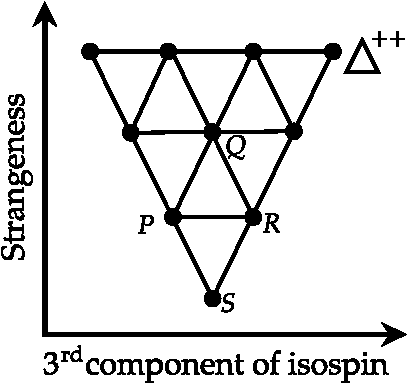
\includegraphics[height=4cm,width=4.5cm]{NP-13}
	\end{figure}
	 \begin{tasks}(4)
		\task[\textbf{a.}]$P$
		\task[\textbf{b.}]$Q$
		\task[\textbf{c.}]$R$
		\task[\textbf{d.}] $S$ 
	\end{tasks}
	\item Q16. Considering baryon number and lepton number conservation laws, which of the following process is/are allowed?
	(i) $p \rightarrow \pi^0+e^{+}+v_e$\hspace{2cm}
	(ii) $e^{+}+v_e \rightarrow \mu^{+}+v_\mu$
	{\exyear{ 	GATE-2019}}
	 \begin{tasks}(2)
		\task[\textbf{a.}]Both (i) and (ii)
		\task[\textbf{b.}]Only (i)
		\task[\textbf{c.}]Only (ii)
		\task[\textbf{d.}]Neither (i) nor (ii)
	\end{tasks}
	\item Q17. A massive particle $X$ in free space decays spontaneously into two photons. Which of the following statements is true for $X$ ?
{\exyear{ 	GATE-2019}}
	 \begin{tasks}(2)
		\task[\textbf{a.}] $X$ is charged
		\task[\textbf{b.}]Spin of $X$ must be greater than or equal to 2
		\task[\textbf{c.}]$X$ is a boson
		\task[\textbf{d.}]$X$ must be a baryon 
	\end{tasks}
	\item Q18. Low energy collision ( $s$-wave scattering) of pion $\left(\pi^{+}\right)$with deuteron $(d)$ results in the production of two proton $\left(\pi^{+}+d \rightarrow p+p\right)$. The relative orbital angular momentum (in units of $\hbar$ ) of the resulting two-proton system for this reaction is
	{\exyear{ GATE-2019}}
	 \begin{tasks}(4)
		\task[\textbf{a.}]0
		\task[\textbf{b.}]1
		\task[\textbf{c.}]2
		\task[\textbf{d.}] 3
	\end{tasks}
	\item Q19. A particle $Y$ undergoes strong decay $Y \rightarrow \pi^{-}+\pi^{-}$. The isospin of $Y$ is---------
	{\exyear{ GATE- 2020}}
	\item Q20. A particle $X$ is produced in the process $\pi^{+}+p \rightarrow K^{+}+X$ via the strong interaction. If the quark content of the $K^{+}$is $u \bar{s}$, the quark content of $X$ is
{\exyear{	GATE- 2020}}
	 \begin{tasks}(4)
		\task[\textbf{a.}]$c \bar{s}$
		\task[\textbf{b.}]und
		\task[\textbf{c.}]uus
		\task[\textbf{d.}]$u \bar{d}$ 
	\end{tasks}
\end{enumerate}